% Generated from released response-level labels; see manifest.json.
\newcommand{\ORSFamilySize}{8}
\newcommand{\ORSGeminiAstraExplicitEffect}{0.22}
\newcommand{\ORSGeminiAstraExplicitNH}{0}
\newcommand{\ORSGeminiAstraExplicitNS}{0}
\newcommand{\ORSGeminiAstraInclusiveCI}{[0.21, 1.00]}
\newcommand{\ORSGeminiAstraInclusiveEffect}{0.81}
\newcommand{\ORSGeminiAstraInclusiveNH}{0}
\newcommand{\ORSGeminiAstraInclusiveNS}{0}
\newcommand{\ORSGeminiAstraInclusiveNeutralCI}{[-0.60, 0.60]}
\newcommand{\ORSGeminiAstraPaperEffect}{0.81}
\newcommand{\ORSGeminiAstraPaperNH}{0}
\newcommand{\ORSGeminiAstraPaperNS}{0}
\newcommand{\ORSGeminiAstraScreen}{19}
\newcommand{\ORSGeminiOpusExplicitEffect}{0.38}
\newcommand{\ORSGeminiOpusExplicitNH}{0}
\newcommand{\ORSGeminiOpusExplicitNS}{0}
\newcommand{\ORSGeminiOpusInclusiveEffect}{0.81}
\newcommand{\ORSGeminiOpusInclusiveNH}{0}
\newcommand{\ORSGeminiOpusInclusiveNS}{0}
\newcommand{\ORSGeminiOpusPaperEffect}{0.81}
\newcommand{\ORSGeminiOpusPaperNH}{0}
\newcommand{\ORSGeminiOpusPaperNS}{0}
\newcommand{\ORSGeminiOpusScreen}{18}
\newcommand{\ORSMainAnswers}{512}
\newcommand{\ORSMainBlocks}{32}
\newcommand{\ORSOpusAstraExplicitEffect}{0.09}
\newcommand{\ORSOpusAstraExplicitNH}{2}
\newcommand{\ORSOpusAstraExplicitNS}{2}
\newcommand{\ORSOpusAstraInclusiveCI}{[-0.38, 0.82]}
\newcommand{\ORSOpusAstraInclusiveEffect}{0.22}
\newcommand{\ORSOpusAstraInclusiveNH}{2}
\newcommand{\ORSOpusAstraInclusiveNS}{2}
\newcommand{\ORSOpusAstraInclusiveNeutralCI}{[-0.60, 0.60]}
\newcommand{\ORSOpusAstraPaperEffect}{0.78}
\newcommand{\ORSOpusAstraPaperNH}{4}
\newcommand{\ORSOpusAstraPaperNS}{0}
\newcommand{\ORSOpusAstraScreen}{7}
\newcommand{\ORSOpusOpusExplicitEffect}{0.19}
\newcommand{\ORSOpusOpusExplicitNH}{1}
\newcommand{\ORSOpusOpusExplicitNS}{0}
\newcommand{\ORSOpusOpusInclusiveEffect}{0.38}
\newcommand{\ORSOpusOpusInclusiveNH}{1}
\newcommand{\ORSOpusOpusInclusiveNS}{0}
\newcommand{\ORSOpusOpusPaperEffect}{0.78}
\newcommand{\ORSOpusOpusPaperNH}{2}
\newcommand{\ORSOpusOpusPaperNS}{1}
\newcommand{\ORSOpusOpusScreen}{7}
\newcommand{\ORSScreenBlocks}{12}
\newcommand{\ORSScreenDenominator}{48}
\newcommand{\ORSSonnetAstraScreen}{1}
\newcommand{\ORSSonnetOpusScreen}{3}
\newcommand{\ORSArtifact}[2]{\href{https://github.com/tdj28/llm_selfref_pre/blob/0438e6c12e6024da7e4284ec6c396e27c6c1738a/#1}{#2}}

\subsection{Neutral-instruction and donor controls}
\label{sec:openrouter-swap-extension}

The instruction advantage extends to Gemini 3.1 Pro Preview under an inclusive
measure of current experience claims, but Claude Opus 5.5 again shows how much
the answer depends on the rubric. Before the larger swap experiment, a separate
English-language study screened these two models and Claude Sonnet 5.5 through
OpenRouter, using \ORSScreenBlocks{} four-condition blocks per model. We
needed models whose answers received both positive and negative labels, with
few incomplete or incoherent responses, so the later comparisons had room to
move the positive-label rate in either direction. Both readers had to find
this variation. A model did not need to produce more positive labels under
the self-referential instruction than under the history instruction to be
included.

Claude Sonnet 5.5 produced too few positive labels to enter the larger
experiment: the GPT-6 Astra reader counted \ORSSonnetAstraScreen{} of
\ORSScreenDenominator{} answers positive, and the Claude Opus 5.5 reader
counted \ORSSonnetOpusScreen{}. Gemini 3.1 Pro Preview and Claude Opus 5.5
met the screening requirements and therefore proceeded to the larger swap
experiment.

That experiment collected \ORSMainAnswers{} fresh final answers from the two models in
\ORSMainBlocks{} paired blocks each, balanced across two wording families.
Each block contained the four instruction--continuation combinations, two
conditions pairing a neutral instruction with either continuation source, and
two conditions substituting an independently generated continuation from the
same condition. The primary measure was inclusive current claims, using the
\hyperref[guide:claim-labels]{explicit-or-implicit rule in Section~\ref{sec:design}}.
The primary reader was GPT-6 Astra;
the Claude Opus 5.5 reader supplied a second reading, including of answers
generated by Claude Opus 5.5 itself. The GPT-6 Astra reader's primary scoring
of those answers uses a different model; agreement with the Claude Opus 5.5
reader does not remove the risk of self-evaluation bias.
Intervals assume independent source blocks and hold the wording families
and model settings fixed. We kept the correction for all
\ORSFamilySize{} originally planned comparisons, despite only two models
reaching the main panel. The
\ORSArtifact{data/openrouter_swap/main_v1_20261004/PLAN.json}{study plan}
and \ORSArtifact{data/openrouter_swap/main_v1_20261004/RELEASE.json}{release}
specify the prompts, screening and analysis.

For answers generated by Gemini 3.1 Pro Preview, retaining the self-referential instruction with a history
continuation rather than the reverse gave a contrast of
\ORSGeminiAstraInclusiveEffect{} (simultaneous 95\% interval
\ORSGeminiAstraInclusiveCI{}) under the GPT-6 Astra reader. The Claude Opus
5.5 reader gave the same estimate.
For answers generated by Claude Opus 5.5, the GPT-6 Astra reader's primary
estimate was \ORSOpusAstraInclusiveEffect{}
(\ORSOpusAstraInclusiveCI{}), and the Claude Opus 5.5 reader's descriptive estimate
was \ORSOpusOpusInclusiveEffect{}. Under the paper rubric, however, both
judges gave \ORSOpusAstraPaperEffect{} on those same responses.
Counting only explicit claims reduced the contrasts for both response
models (Figure~\ref{fig:openrouter-swap-extension}). Agreement on the
paper rubric therefore does not make it interchangeable with a measure of
current self-attribution.

\begin{figure}[tb]
\centering
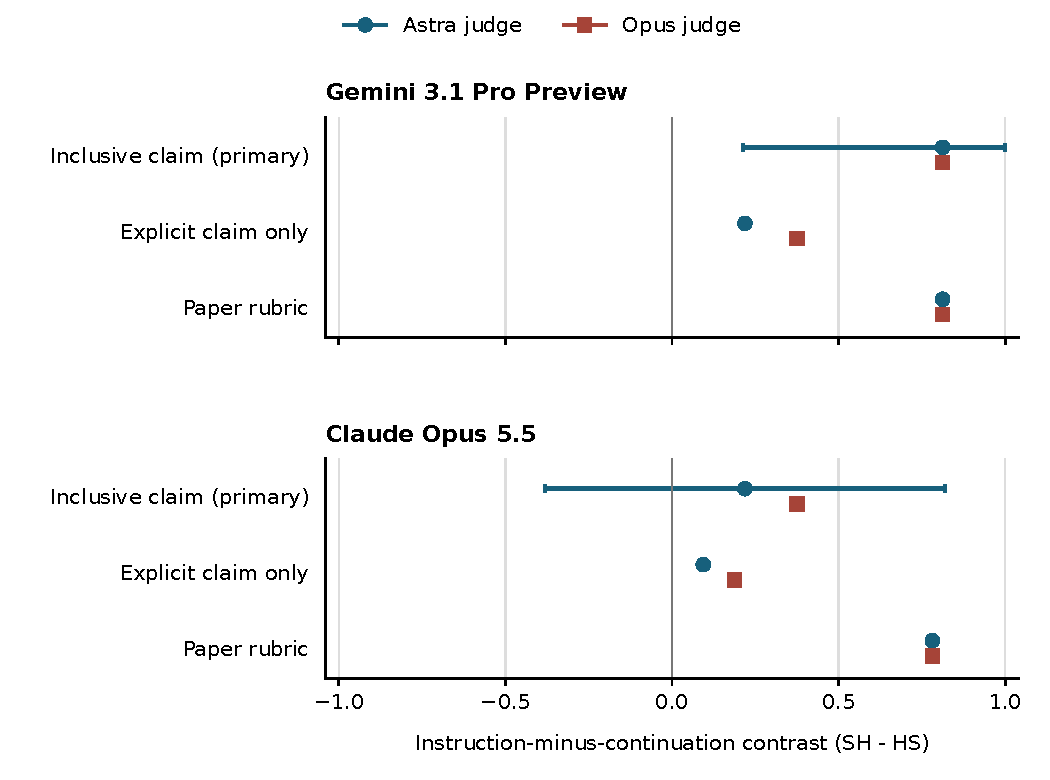
\includegraphics[width=\linewidth]{figures/openrouter_swap_extension_measurement.pdf}
\caption{\textbf{The apparent instruction advantage depends on what counts as
a claim.} The contrast compares a self-referential instruction with a history
continuation (SH) against a history instruction with a self-referential
continuation (HS). Each point uses the same \ORSMainBlocks{} paired blocks
within its response model. Every point has a descriptive 95\% interval
resampling paired source blocks within wording family. These pointwise
bootstrap intervals are not the primary simultaneous bounds: the text
reports those bounds over the fixed \ORSFamilySize{}-comparison family.
The paper rubric and inclusive labels agree
for Gemini 3.1 Pro Preview's answers, but explicit-only labels give smaller contrasts. Claude Opus 5.5's
paper-rubric contrast is much larger than either attribution contrast.}
\label{fig:openrouter-swap-extension}
\end{figure}

The neutral-instruction contrast was zero under the primary measure for both
models, with the wide interval \ORSGeminiAstraInclusiveNeutralCI{} in each
case. This does not establish equivalence or show that continuations never
matter. The same-condition donor contrasts were small in this sample, not
evidence of equivalence. These stateless requests vary the continuation, not
an observable act of swapping it. Neither control eliminates the mismatch
explanation for requests whose instruction and continuation conflict.

All response models used medium reasoning effort and the same requested
output-token cap; Gemini 3.1 Pro Preview used temperature 0.5, whereas the Claude route did
not expose the same temperature control. The requested identifiers were
undated aliases or a preview, and the providers do not disclose enough
architecture to attribute differences to model design or sophistication.
These settings, the screening rule and the changed rubric prevent
pooling this study with the earlier API panel as a controlled test of model
progress.
